\documentclass[border=4pt]{standalone}
\usepackage{tikz}
\usetikzlibrary{positioning, arrows.meta, shapes.geometric, calc, fit, backgrounds}
\usepackage{amsmath,amssymb}

\pgfdeclarelayer{background}
\pgfsetlayers{background,main}

\begin{document}
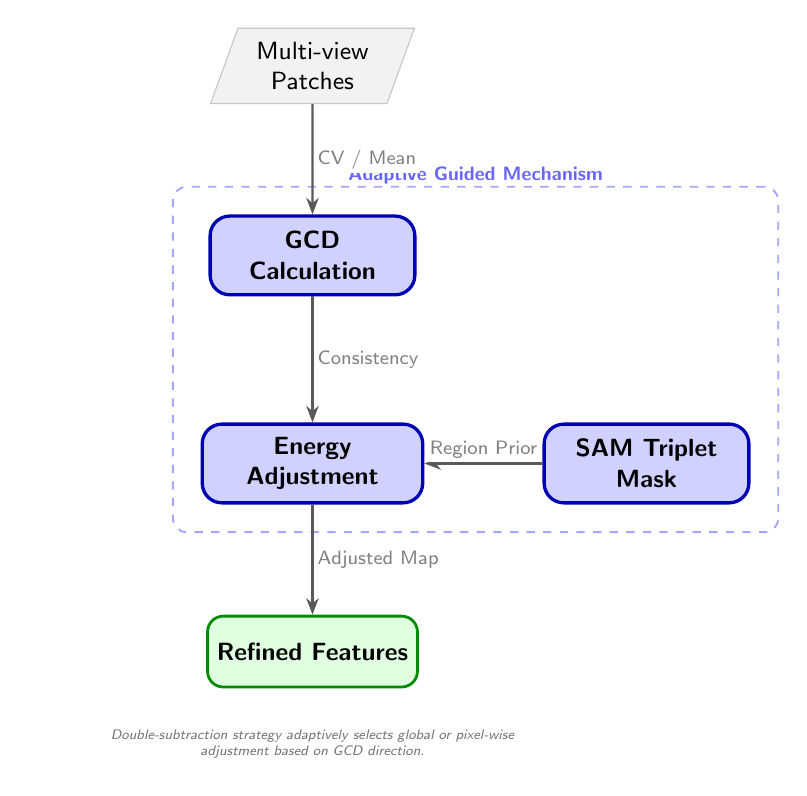
\begin{tikzpicture}[
  input/.style={draw, trapezium, trapezium left angle=70, trapezium right angle=110,
                minimum width=2.6cm, minimum height=0.7cm, fill=gray!10, draw=gray!45, align=center,
                font=\sffamily\small},
  innov/.style={draw, rounded corners=2.5mm, minimum width=2.6cm, minimum height=1.0cm,
                fill=blue!18, draw=blue!70!black, line width=1.2pt, align=center,
                font=\sffamily\small\bfseries},
  output/.style={draw, rounded corners=2mm, minimum width=2.6cm, minimum height=0.9cm,
                 fill=green!12, draw=green!55!black, line width=1pt, align=center,
                 font=\sffamily\small\bfseries},
  arr/.style={-{Stealth[length=6pt]}, thick, color=black!65},
  lbl/.style={font=\sffamily\scriptsize, text=black!50, fill=white, inner sep=1.5pt},
  gbox/.style={draw=blue!35, dashed, rounded corners=5pt, inner sep=10pt, line width=0.7pt},
]

% Input
\node[input] (m1) {Multi-view\\Patches};

% GCD Calculation
\node[innov, below=1.4cm of m1] (m2) {GCD\\Calculation};

% Energy Adjustment (main column)
\node[innov, below=1.6cm of m2, minimum width=2.8cm] (m4) {Energy\\Adjustment};

% SAM Triplet Mask (side input)
\node[innov, right=1.5cm of m4] (m3) {SAM Triplet\\Mask};

% Output
\node[output, below=1.4cm of m4] (m5) {Refined Features};

% Arrows
\draw[arr] (m1) -- node[lbl, right] {CV / Mean} (m2);
\draw[arr] (m2) -- node[lbl, right] {Consistency} (m4);
\draw[arr] (m3) -- node[lbl, above] {Region Prior} (m4);
\draw[arr] (m4) -- node[lbl, right] {Adjusted Map} (m5);

% Group box
\begin{scope}[on background layer]
\node[gbox, fit=(m2)(m3)(m4),
      label={[font=\sffamily\scriptsize\bfseries, text=blue!60, yshift=-3pt]above:Adaptive Guided Mechanism}] {};
\end{scope}

% Annotation
\node[font=\sffamily\tiny\itshape, text=black!55, below=0.4cm of m5, text width=7cm, align=center]
   {Double-subtraction strategy adaptively selects global or pixel-wise\\adjustment based on GCD direction.};

\end{tikzpicture}
\end{document}